%!TEX TS-program = xelatex
%!TEX encoding = UTF-8 Unicode

%%
%% 计算复杂性基础作业模板,参考 https://github.com/heygrain/LaTeXTemp 修改而成
%% This work is licensed under a [CC BY-NC-SA 4.0](http://creativecommons.org/licenses/by-nc-sa/4.0/). The author is [Arpe1s](https://blog.arpe1s.xyz/).
%% 

%% 设置纸张类型、文字大小、文档类型
\documentclass[a4paper, 12pt]{article}

%% 导入需要用的包
\usepackage{xeCJK} % 支持中文,我觉得比 \usepackage[UTF8]{ctex} 漂亮
% \usepackage[UTF8]{ctex}
\usepackage{verbatim} % 支持多行注释等原文照排功能
\usepackage{color} % 支持彩色文字
\usepackage{cite} % 支持参考文献
\usepackage[backref]{hyperref} % 支持超链接
\usepackage{amssymb, amsfonts, amsmath, amsthm} % 支持美国数学学会的数学符号字体库

%% 图形相关包
\usepackage[x11names]{xcolor} % 颜色
\usepackage{graphicx} % 处理图片
\usepackage{pstricks, pst-plot, pst-eps} % 绘图
\usepackage{subfig} % 子图
\def\pgfsysdriver{pgfsys-dvipdfmx.def} % put before tikz
\usepackage{tikz} % 绘图

%% 段落格式相关包
\usepackage{indentfirst} % 支持首段缩进
\setlength{\parindent}{2.1em}
\renewcommand{\baselinestretch}{1.4} % 1.4倍行距
\usepackage[a4paper]{geometry} % 页边距
\geometry{
    verbose,
    tmargin=3cm,% 上边距
    bmargin=3cm,% 下边距
    lmargin=3cm,% 左边距
    rmargin=3cm % 右边距
}
\setlength{\parskip}{0.4ex} % 段落间距
\usepackage{enumitem} % 调整列表间距
\setenumerate[1]{itemsep=0pt, partopsep=0pt, parsep=\parskip, topsep=5pt}
\setitemize[1]{itemsep=0.4ex, partopsep=0.4ex, parsep=\parskip, topsep=0.4ex}
\setdescription{itemsep=0pt, partopsep=0pt, parsep=\parskip, topsep=5pt}

%% 自定义新命令
\newcommand{\horrule}[1]{\rule[0.5ex]{\linewidth}{#1}} 	% 画水平线

%% 更改以适应中文,若使用 \usepackage[UTF8]{ctex} 则不需要改
\renewcommand{\refname}{参考文献}
\renewcommand{\abstractname}{\large \bf 摘\quad 要}
\renewcommand{\contentsname}{目录}
\renewcommand{\tablename}{表}
\renewcommand{\figurename}{图}

%% 定理、公理、引理、命题、推论、注相关配置
\newtheorem{theorem}{\hspace{2em}定理}[section]
\newtheorem{axiom}{\hspace{2em}公理}[section] 
\newtheorem{lemma}{\hspace{2em}引理}[section] 
\newtheorem{proposition}{\hspace{2em}命题}[section] 
\newtheorem{corollary}{\hspace{2em}推论}[section] 
\newtheorem{remark}{\hspace{2em}注}[section]

%% 使封面的作者信息居中后左对齐
\usepackage{titling}
\preauthor{
    \begin{center} % 居中环境,左对齐环境为 flushleft
    \large \lineskip 1em%
    \begin{tabular}[t]{l} % 左对齐
}
\postauthor{
    \end{tabular} \par % 分段
    \end{center}
}

%%%%%%%%%%%%%%%%%%%%%%%%%%%%%%%%%%%%%%%%%%%%%%%%%%%%%%%%%%%%%%%%%%%%%%%%%%%%%%%
% 课程要求及作业要求
\begin{comment}
    课程要求:
    手机关闭/静音;听讲、讨论、笔记、复习、调研、按时完成作业。
    作业要求:
    练习与读书报告,随堂布置。
    读书报告格式包括:摘要、引言、预备知识、主要结果及证明、结论、参考文献。
    布置作业后第二周周日24点前电子版(word或tex文件)发助教邮箱,过期视为未完成。出现雷同或者网络抄袭者,当次作业记为0分。
    成绩总分100分,其中:按时上课10分;作业完成:90分。
    助教:王梦凡 wangmengfan@iie.ac.cn
\end{comment}

% 作业模板说明
\begin{comment}
    这是我参考 \herf{https://github.com/heygrain/LaTeXTemp}{LaTeXTemp} 修改而成的中文作业模板。
    主要用于我的计算复杂性基础课程作业。只能用 XeLaTeX 编译。
    编译时如果超链接等等显示为问号,或者出现参考文献不显示的情况,则需要多编译几次。
    而且有时候需要先用 BibTeX 编译,再用 XeLaTeX 编译才能正确显示。
    具体原因未知,搜索可知网络上存在大量遇到同样问题的,应该是 XeLaTeX 本身的问题。
    助教若遇到编译问题,可以查看我提交的附近里的编译好的 .pdf 文件。
    作业批改时若遇到问题,随时可以联系我,联系方式在正文的标题处有给出。
\end{comment}

%%%%%%%%%%%%%%%%%%%%%%%%%%%%%%%%%%%%%%%%%%%%%%%%%%%%%%%%%%%%%%%%%%%%%%%%%%%%%%%
% 前导命令结束,文本部分开始
\begin{document}

% 设置标题、作者、时间,以及相关格式
\title{
    {
    \begin{figure}[htbp]
        \centering % 居中
        
\includegraphics[width = 0.7 \textwidth]{xgs_logo.png}
    \end{figure}
    }
    {
        \normalfont\normalsize\textsc{
            Institute of Information Engineering \\
            Computational Complexity, Spring 2022 \\
            [25pt]
        }
    }
    \horrule{0.5pt}
    \sffamily{
        计算复杂性基础 \\
        第一次作业 \\
        第一部分 \ \ 六道计算题
    }
    \horrule{1.8pt} \\ [20pt]
}
\author{
    学号:1234567 \\ 
    姓名:小明 \\
    邮箱: 1234567 \\
    联系方式:1234567 \\ [60pt]
}
\date{\today}

%%%%%%%%%%%%%%%%%%%%%%%%%%%%%%%%%%%%%%%%%%%%%%%%%%%%%%%%%%%%%%%%%%%%%%%%%%%%%%%
% 独立的题名封面
\begin{titlepage}
    \maketitle
    \vspace{30pt}
    \thispagestyle{empty} % 去掉页码
\end{titlepage}

% 摘要页
\begin{abstract}
        \normalsize \ \ 这是中文摘要。 \\[5pt]
        \indent \ \ \textbf{关键词}:图灵机、BPP
\end{abstract}
\thispagestyle{empty} % 去掉页码
\newpage

    % 设置目录,切换页码用的字母可以让正文从第一页开始
\pagenumbering{roman}
\tableofcontents
\newpage
\pagenumbering{arabic}

%%%%%%%%%%%%%%%%%%%%%%%%%%%%%%%%%%%%%%%%%%%%%%%%%%%%%%%%%%%%%%%%%%%%%%%%%%%%%%%
% 分节命令,第一节
\section{引言}
这里展示常用中文字体。

默认字体为宋体。{\sffamily 这是黑体。} {\rmfamily 这是宋体。} {\ttfamily 这是仿宋。} {\it 这是楷体。}

或者 \textsf{黑体},\textrm{宋体},\texttt{仿宋},\textit{楷体}。

%%%%%%%%%%%%%%%%%%%%%%%%%%%%%%%%%%%%%%%%%%%%%%%%%%%%%%%%%%%%%%%%%%%%%%%%%%%%%%%
% 分节命令,第二节
\section{预备知识}

% 分节命令,第二节第一小节
\subsection{超链接}
这里展示两种超链接的使用。

\label{sec1}

\href{https://blog.arpe1s.xyz/}{我的博客}

% 分节命令,第二节第二小节
\subsection{文献引用}
这里展示参考文献引用的方法 \cite{LMZ1999}。

下面展示定理的用法。

\begin{theorem}[地圆说]
    \label{thm: thm1}
    地球不是平面。
\end{theorem}

引用定理 ~\ref{thm: thm1}。

%%%%%%%%%%%%%%%%%%%%%%%%%%%%%%%%%%%%%%%%%%%%%%%%%%%%%%%%%%%%%%%%%%%%%%%%%%%%%%%
% 分节命令,第三节
\section{主要结果及证明}
第二节第一小节的超链接 ~\ref{sec1} 以及页面链接 ~\pageref{sec1}。

下面展示行内公式和多行公式的写法。

\[ \frac{2}{3} = 2 \div 3 \]

\begin{eqnarray}
    \label{eqn: eqn1}
    a & = & b + c \\
      & = & y - z
\end{eqnarray}

引用公式 ~\ref{eqn: eqn1}。

%%%%%%%%%%%%%%%%%%%%%%%%%%%%%%%%%%%%%%%%%%%%%%%%%%%%%%%%%%%%%%%%%%%%%%%%%%%%%%%
% 分节命令,第四节
\section{结论}
这里展示图和表的用法。

% 分节命令,第四节第一小节
\subsection{图}
\begin{figure}[ht]
    \centering
    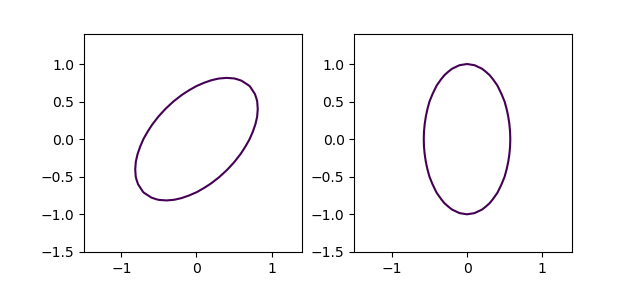
\includegraphics[width = \textwidth]{example.png}
    \caption{这是一个图}
    \label{fig: fig1}
\end{figure}

引用图 ~\ref{fig: fig1}。

% 分节命令,第四节第二小节
\subsection{表}
\begin{table}[ht] % 调节图片位置,h:浮动;t:顶部;b:底部;p:当前位置
    \caption{这是一个表}
    \label{tb: filter}
    \centering
    \begin{tabular}{cccc} % 表格中的数据居中,c 的个数为表格的列数
        \hline
        & 卡尔曼滤波 & 神经网络滤波 & 被动无源滤波 \\ 
        \hline
        模型类型 & 线性 & 线性 & 非线性 \\ 
        参数调校 & 大量 & 几乎没有 & 合理 \\ 
        稳定性 & 满足全局稳定性 & 依赖于模型 & 满足子系统稳定性 \\ 
        \hline
        \end{tabular} 
\end{table}

引用表格 ~\ref{tb: filter}。

%%%%%%%%%%%%%%%%%%%%%%%%%%%%%%%%%%%%%%%%%%%%%%%%%%%%%%%%%%%%%%%%%%%%%%%%%%%%%%%
% 参考文献
\bibliographystyle{plain}
\bibliography{references.bib}

% 文本结束
\end{document}